\label{ch:push}
\section{Push Notification Service}
Eine Notification dient dazu den Benutzer über etwas zu informieren. Dies kann ein Kalender-Eintrag, eine eingetroffene SMS-Nachricht oder ein anderes Ereignis sein. Diese Art der Benachrichtigung wird meist über eine Local Notification erzeugt. Eine Local Notification wird aufgrund eines lokal am Gerät auftretenden Ereignisses ausgelöst. Ein Beispiel ist in Abbildung \ref{fig:local-notification} zu sehen.
\begin{figure}
    \centering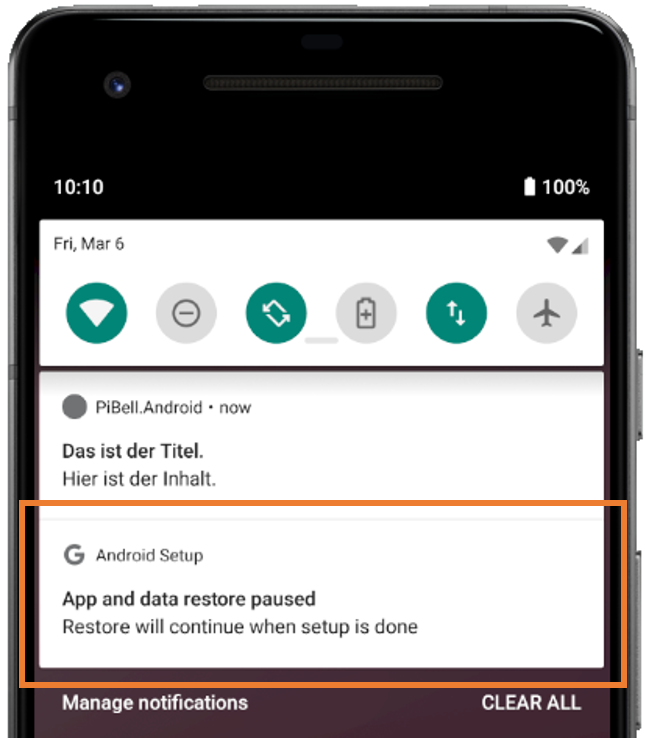
\includegraphics[width=.5\linewidth]{images/xamarin/LocalNotification.png}
    \caption{Lokale Benachrichtigung}
    \label{fig:local-notification}
\end{figure}

Im Gegensatz dazu dient eine Push Notification dazu, ein externes Ereignis auf einem anderen Gerät zu verarbeiten.
Das Empfängergerät zeigt dem Benutzer in den meisten Fällen eine zusätzliche Local Notification an.
Beispiele für Push Notifications sind Katastrophenwarnungen, neue Instant-Messenger-Nachrichten, oder ähnliche Ereignisse, die nicht auf dem Empfängegerät ihren Ursprung haben.

\subsection{Funktionsweise}
Eine Push Notification wird immer von einem sogenannten Push Notification Service an alle Zielgeräte geschickt.
Dieser Service wird vom jeweiligen Betriebssystem-Hersteller bereitgestellt.
Im Fall der hier entwickelten App sind das Google und Apple, mit ihren Push Notification Services \ac{gcm} und \ac{apns}.\par

Der Service ist dafür verantwortlich, die Benachrichtigung an alle registrierten Zielgeräte zu schicken.
Wenn das Zustellen nicht möglich ist, bricht der Service die Zustellung nach mehreren Versuchen für dieses Gerät ab.
Alle anderen Geräte erhalten die Benachrichtigung.
Daher ist es nicht sichergestellt, dass eine Push-Benachrichtigung bei jedem Gerät ankommt.\par

Zusätzlich zum Nachrichtentext können bei einer Push Notification zusätzliche Daten mitgeschickt werden. Diese können zum Beispiel die App über die genaue Benachrichtigungsursache informieren.

\section{AppCenter Push}
AppCenter Push hat in erster Linie die Funktion, den Zugriff auf die verschiedenen Push Notification Services zu vereinheitlichen und damit einfacher zu gestalten.
Microsoft AppCenter verwaltet alle Server-\ac{api}-Schlüssel, Zielgerätelisten und ähnliche Einstellungen, um den Prozess des Benachrichtigung-Sendens zu vereinfachen.
AppCenter Push ist entweder über das Web-Interface unter \url{https://appcenter.ms/} oder über die AppCenter \ac{api} erreichbar und verwendbar.\par

Die AppCenter Push \ac{sdk} abstrahiert den ganzen Prozess der Geräte-Registration, sowie der Registrierung des Eingangs-Events und versteckt alles hinter einer einzelnen simplen Funktion \texttt{AppCenter.Start(„{App Secret}“, typeof(Push));}.
Das App Secret ist der von AppCenter zugewiesene Schlüssel mit dem sichergestellt wird, dass das Gerät für das richtige AppCenter Projekt registriert wird.
Ohne diese \ac{sdk} müsste in der App viel mehr konfiguriert werden, was einen höheren Programmieraufwand und größere Fehlerraten zur Folge hat.
Außerdem würde das Rad neu erfunden werden.\par

In der entwickelten App wird die AppCenter-\ac{sdk}-Version 2.6.4 verwendet. Zu beachten ist, dass AppCenter Push nicht mehr weiterentwickelt und irgendwann dieses Jahr der Service abgeschaltet wird, wie es John Wargo in seinem Blog-Post am 3. Februar 2020 geschrieben hat. Bevor AppCenter Push endgültig terminiert wird, will Microsoft detaillierte Anleitungen zum Umstieg auf Azure bereitstellen.